        \documentclass{standalone}
        \usepackage{tikz}
        \begin{document}
        \fontsize{16px}{16px}\selectfont
        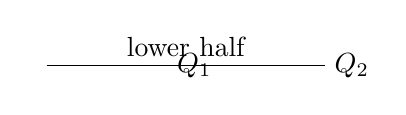
\begin{tikzpicture}


    \node at (0,0) (nodeA) {};
    \node at (2,0) (nodeB) {$Q_1$};
    \node at (4,0) (nodeC) {$Q_2$};
    \draw (nodeA) -- (nodeC) node [midway, above] (TextNode) {lower half};
    \draw (nodeA) -- (nodeB);
    \draw (nodeB) -- (nodeC);
        \end{tikzpicture}
        \end{document}
